\documentclass[conference,a4paper]{IEEEtran}
\usepackage[utf8]{inputenc}
\usepackage[T1]{fontenc}
\usepackage{amsmath,amssymb}
\usepackage{graphicx}
\usepackage{booktabs}
\usepackage{url}
\usepackage{cite}
\usepackage{array}
\usepackage{microtype}
\graphicspath{{../outputs/}}

\title{Perbandingan CNN Baseline, CNN dengan Dropout, dan ResNet-18 Transfer Learning untuk Klasifikasi Citra CIFAR-10}

\author{\IEEEauthorblockN{Ahmad Furqon Ramadhani}
\IEEEauthorblockA{Program Studi Teknik Informatika\\
Universitas Darussalam Gontor\\
NIM: 452024611066\\
Email: afurqonramadhani24@student.cs.unida.gontor.ac.id}}

\begin{document}
\maketitle

\begin{abstract}
Klasifikasi citra merupakan salah satu penerapan utama deep learning karena model dapat mempelajari representasi visual secara hierarkis dari data. Penelitian ini membandingkan CNN sederhana sebagai baseline, CNN dengan dropout, dan ResNet-18 pretrained dengan transfer learning pada dataset CIFAR-10. Dataset terdiri atas 60.000 citra RGB berukuran 32x32 piksel dalam 10 kelas. Sebanyak 45.000 citra digunakan untuk training, 5.000 untuk validation, dan 10.000 untuk testing. Tiga skenario eksperimen dirancang dengan optimizer Adam: E1 CNN baseline dengan learning rate 0,001, E2 CNN dengan dropout 0,5 dan learning rate 0,001, serta E3 ResNet-18 pretrained dengan learning rate 0,0001. Training menggunakan batch size 128, maksimum 20 epoch, seed 42, dan early stopping berdasarkan validation loss dengan patience 5. Evaluasi menggunakan loss, accuracy, precision, recall, F1-score, training curves, dan confusion matrix. Hasil test menunjukkan E1 memperoleh accuracy 68,92% dan F1 68,53%, E2 67,39% dan 67,22%, sedangkan E3 mencapai 95,22% untuk accuracy dan F1. Analisis training menunjukkan E1 dan E2 belajar relatif stabil tanpa overfitting berat, sementara E3 mulai menunjukkan gap train-validation setelah sekitar epoch 7 dan dihentikan lebih awal pada epoch 12. Confusion matrix juga menunjukkan kesalahan E1 dan E2 lebih banyak terkonsentrasi pada kelas hewan, sedangkan E3 memiliki diagonal yang jauh lebih dominan. Hasil ini menunjukkan bahwa transfer learning berbasis ResNet-18 memberikan representasi yang lebih efektif daripada CNN sederhana pada konfigurasi CIFAR-10 yang digunakan.
\end{abstract}

\begin{IEEEkeywords}
deep learning, computer vision, CIFAR-10, convolutional neural network, dropout, ResNet-18, transfer learning.
\end{IEEEkeywords}

\section{Introduction}
Klasifikasi citra merupakan masalah penting dalam computer vision dan menjadi salah satu domain utama pembelajaran mendalam. Convolutional Neural Network (CNN) memanfaatkan operasi konvolusi untuk mempelajari pola lokal dan membangun representasi hierarkis dari citra, sehingga berhasil digunakan pada banyak tugas pengenalan visual. Namun, performa CNN sederhana dapat terbatas ketika kompleksitas data meningkat.

Salah satu pendekatan untuk meningkatkan generalisasi model adalah regularisasi, salah satunya dropout. Dropout bekerja dengan menonaktifkan unit secara acak selama training sehingga mengurangi co-adaptation dan dapat membantu mengendalikan overfitting [1]. Pendekatan lain yang lebih kuat adalah transfer learning, yaitu memanfaatkan representasi yang telah dipelajari pada domain sumber kemudian mengadaptasinya pada tugas target [2]. ResNet memperkenalkan residual learning untuk mempermudah optimasi jaringan yang lebih dalam dan menghasilkan representasi visual yang kuat [3].

Penelitian ini menggunakan CIFAR-10 sebagai studi kasus karena memiliki 10 kelas citra berwarna dengan ukuran kecil dan distribusi kelas yang seimbang [4]. Tujuan penelitian adalah membandingkan tiga konfigurasi: CNN baseline, CNN dengan dropout 0,5, dan ResNet-18 pretrained melalui transfer learning. Pertanyaan penelitian yang ingin dijawab adalah: (1) apakah dropout meningkatkan generalisasi CNN sederhana; (2) seberapa besar keuntungan transfer learning dibandingkan CNN baseline; dan (3) konfigurasi mana yang memberikan keseimbangan terbaik antara performa test dan perilaku training.

Penelitian menyediakan perbandingan eksperimen, analisis training dan overfitting, serta error analysis berbasis confusion matrix dari training nyata di GPU Google Colab.

\section{Related Work}
CNN merupakan fondasi penting dalam pengenalan citra karena mampu mempelajari fitur visual secara hierarkis [3]. Seiring meningkatnya kedalaman jaringan, proses optimasi dapat menjadi lebih sulit. He \textit{et al.} memperkenalkan residual learning pada ResNet untuk membuat jaringan dalam lebih mudah dioptimalkan [3]. Arsitektur tersebut kemudian banyak digunakan sebagai backbone untuk berbagai tugas computer vision.

Dropout merupakan salah satu regularisasi yang populer untuk mengurangi overfitting. Srivastava \textit{et al.} menunjukkan bahwa random unit dropping dapat mengurangi co-adaptation dan meningkatkan generalisasi pada jaringan neural [1]. Dalam penelitian ini dropout diuji secara eksplisit pada baseline CNN agar pengaruh regularisasi dapat dibandingkan langsung.

Transfer learning menyediakan mekanisme untuk memanfaatkan pengetahuan yang diperoleh dari domain sumber pada tugas baru. Pan dan Yang membahas transfer learning sebagai pendekatan untuk memindahkan pengetahuan ketika distribusi atau ruang fitur antar-domain berbeda [2]. Pada penelitian ini, ResNet-18 menggunakan bobot pretrained ImageNet kemudian dilakukan fine-tuning pada CIFAR-10.

Optimasi model dilakukan dengan Adam, yang menggunakan estimasi momen pertama dan kedua gradien untuk mengatur langkah pembaruan parameter secara adaptif [5].

\section{Methodology}
\subsection{Dataset}
CIFAR-10 terdiri atas 60.000 citra RGB berukuran 32x32 piksel yang terbagi menjadi 10 kelas: airplane, automobile, bird, cat, deer, dog, frog, horse, ship, dan truck. Dataset menyediakan 50.000 citra training dan 10.000 citra testing; setiap kelas memiliki 5.000 citra training dan 1.000 citra testing pada pembagian resminya [4].

Implementasi penelitian membagi 50.000 citra training menjadi 45.000 citra training dan 5.000 citra validation menggunakan random split dengan seed 42. Pembagian ini dilakukan hanya dari split training asli, sedangkan 10.000 citra test dipertahankan sebagai data pengujian akhir. Dengan demikian tidak terdapat penggunaan data test selama proses training.

\subsection{Preprocessing}
Untuk E1 dan E2, citra dipertahankan pada resolusi 32x32 dengan random horizontal flip dan random crop 32x32 pada training. Data validation dan test tidak menerima augmentasi. Normalisasi menggunakan mean CIFAR-10 $(0.4914,0.4822,0.4465)$ dan standar deviasi $(0.2470,0.2435,0.2616)$.

Untuk E3, citra diubah menjadi 224x224 agar sesuai dengan input ResNet-18 pretrained. Training menggunakan random horizontal flip, random crop 224x224 dengan padding 8, kemudian normalisasi ImageNet $(0.485,0.456,0.406)$ dengan standar deviasi $(0.229,0.224,0.225)$. Validation dan test menggunakan resize 224x224 tanpa augmentation. Pendekatan ini memastikan preprocessing kompatibel dengan bobot pretrained.

\subsection{Baseline CNN}
Baseline menggunakan CNN sederhana yang terdiri atas tiga blok konvolusi berturut-turut dengan jumlah channel 32, 64, dan 128. Setiap konvolusi diikuti ReLU dan max pooling pada dua blok awal, kemudian adaptive average pooling dan lapisan linear untuk klasifikasi 10 kelas. E1 menggunakan dropout 0,0 sehingga menjadi baseline murni.

\subsection{ResNet-18 Transfer Learning}
Model utama menggunakan ResNet-18 pretrained. Lapisan klasifikasi terakhir diganti menjadi linear layer dengan 10 keluaran untuk CIFAR-10. Seluruh parameter model di-fine-tune menggunakan data target. ResNet-18 dipilih karena residual learning membantu optimasi jaringan yang lebih dalam dan transfer learning memanfaatkan representasi yang sudah dipelajari [2], [3].

\subsection{Loss dan Optimasi}
Semua eksperimen menggunakan categorical cross-entropy melalui `CrossEntropyLoss`. Secara umum loss dihitung sebagai
\begin{equation}
L=-\frac{1}{N}\sum_{i=1}^{N}\log p(y_i\mid x_i),
\end{equation}
where $p(y_i\mid x_i)$ adalah probabilitas prediksi kelas yang benar. Optimasi menggunakan Adam [5].

\section{Experimental Setup}
Tiga skenario eksperimen dirancang sesuai requirement tugas: satu baseline, satu variasi regularisasi, dan satu model utama berbasis transfer learning. Konfigurasi utama disajikan pada Tabel I.

\begin{table}[htbp]
\caption{Konfigurasi Eksperimen}
\centering
\begin{tabular}{lcccc}
\toprule
Eksperimen & Model & Dropout & LR & Pretrained \\
\midrule
E1 & CNN baseline & 0,0 & 0,001 & Tidak \\
E2 & CNN + Dropout & 0,5 & 0,001 & Tidak \\
E3 & ResNet-18 & -- & 0,0001 & Ya \\
\bottomrule
\end{tabular}
\label{tab:exp}
\end{table}

Training menggunakan batch size 128 dan maksimum 20 epoch pada GPU NVIDIA Tesla T4 di Google Colab. Seed 42 digunakan untuk menjaga reproducibility. Early stopping menggunakan patience 5 berdasarkan validation loss, dan checkpoint terbaik disimpan berdasarkan validation loss terendah. E1 dan E2 menyelesaikan 20 epoch, sedangkan E3 berhenti pada epoch 12 setelah lima epoch berturut-turut tidak menghasilkan perbaikan validation loss.

Metrik evaluasi meliputi accuracy, precision, recall, dan F1-score dengan macro averaging. Selain metrik test, proses training dianalisis menggunakan training loss, validation loss, training accuracy, validation accuracy, dan confusion matrix. Source code serta hasil eksperimen disediakan pada repository: \url{https://github.com/xygritte/ML2-UAS-Individual-Deep-Learning-Research-Project}.

\section{Results and Discussion}
\subsection{Quantitative Results}
Hasil akhir test ditunjukkan pada Tabel II. Semua nilai berasal dari eksperimen yang benar-benar dijalankan dengan checkpoint terbaik berdasarkan validation loss.

\begin{table}[htbp]
\caption{Hasil Evaluasi Test}
\centering
\begin{tabular}{lccccc}
\toprule
Eksperimen & Loss & Acc. & Prec. & Recall & F1 \\
\midrule
E1 & 0,9078 & 68,92\% & 70,16\% & 68,92\% & 68,53\% \\
E2 & 0,9396 & 67,39\% & 68,12\% & 67,39\% & 67,22\% \\
E3 & \textbf{0,1549} & \textbf{95,22\%} & \textbf{95,23\%} & \textbf{95,22\%} & \textbf{95,22\%} \\
\bottomrule
\end{tabular}
\label{tab:results}
\end{table}

E3 memberikan peningkatan accuracy sebesar 26,30 poin persentase dibandingkan E1 dan 27,83 poin dibandingkan E2. Selisih tersebut menunjukkan bahwa pretrained residual representation memberikan keuntungan yang jauh lebih besar daripada perubahan dropout pada baseline CNN untuk konfigurasi eksperimen ini. E2 justru sedikit lebih rendah daripada E1, sehingga dropout 0,5 tidak dapat dikatakan meningkatkan performa pada konfigurasi tersebut.

\begin{table}[htbp]
\caption{Ringkasan Perilaku Training}
\centering
\begin{tabular}{lccc}
\toprule
Eksperimen & Epoch terbaik val. & Val. Acc. & Epoch terakhir \\
\midrule
E1 & 20 & 68,50\% & 20 \\
E2 & 19 & 66,36\% & 20 \\
E3 & 7 & 95,74\% & 12 \\
\bottomrule
\end{tabular}
\label{tab:training}
\end{table}

\subsection{Training Analysis}
E1 meningkat dari 30,70\% menjadi 69,26\% training accuracy, sementara validation accuracy mencapai 68,50\%. Gap train-validation yang kecil menunjukkan tidak ada overfitting berat, tetapi performa di bawah 70\% menunjukkan keterbatasan baseline [1].

E2 meningkat dari 26,81\% menjadi 62,82\% training accuracy, dengan validation accuracy 66,26\% pada epoch 20. Dropout tidak meningkatkan test, sehingga regularisasi 0,5 belum memberi keuntungan pada baseline ini.

E3 mencapai validation accuracy 95,74\% pada epoch 7 saat training accuracy 98,92\%. Setelah itu training accuracy mendekati 99\% sementara validation accuracy berfluktuasi dan validation loss meningkat. Pola ini menunjukkan overfitting ringan. Early stopping menghentikan training pada epoch 12.

\subsection{Error Analysis}
Confusion matrix E1 dan E2 memperlihatkan lebih banyak massa di luar diagonal pada kelas-kelas hewan. Kesalahan yang paling terlihat secara visual terjadi pada kelompok bird, cat, dog, deer, dan frog, yang memiliki kemiripan bentuk dan tekstur pada resolusi 32x32. E2 mempertahankan pola kesalahan yang mirip sehingga dropout tidak mengubah sumber error utama.

\begin{figure}[htbp]
\centering
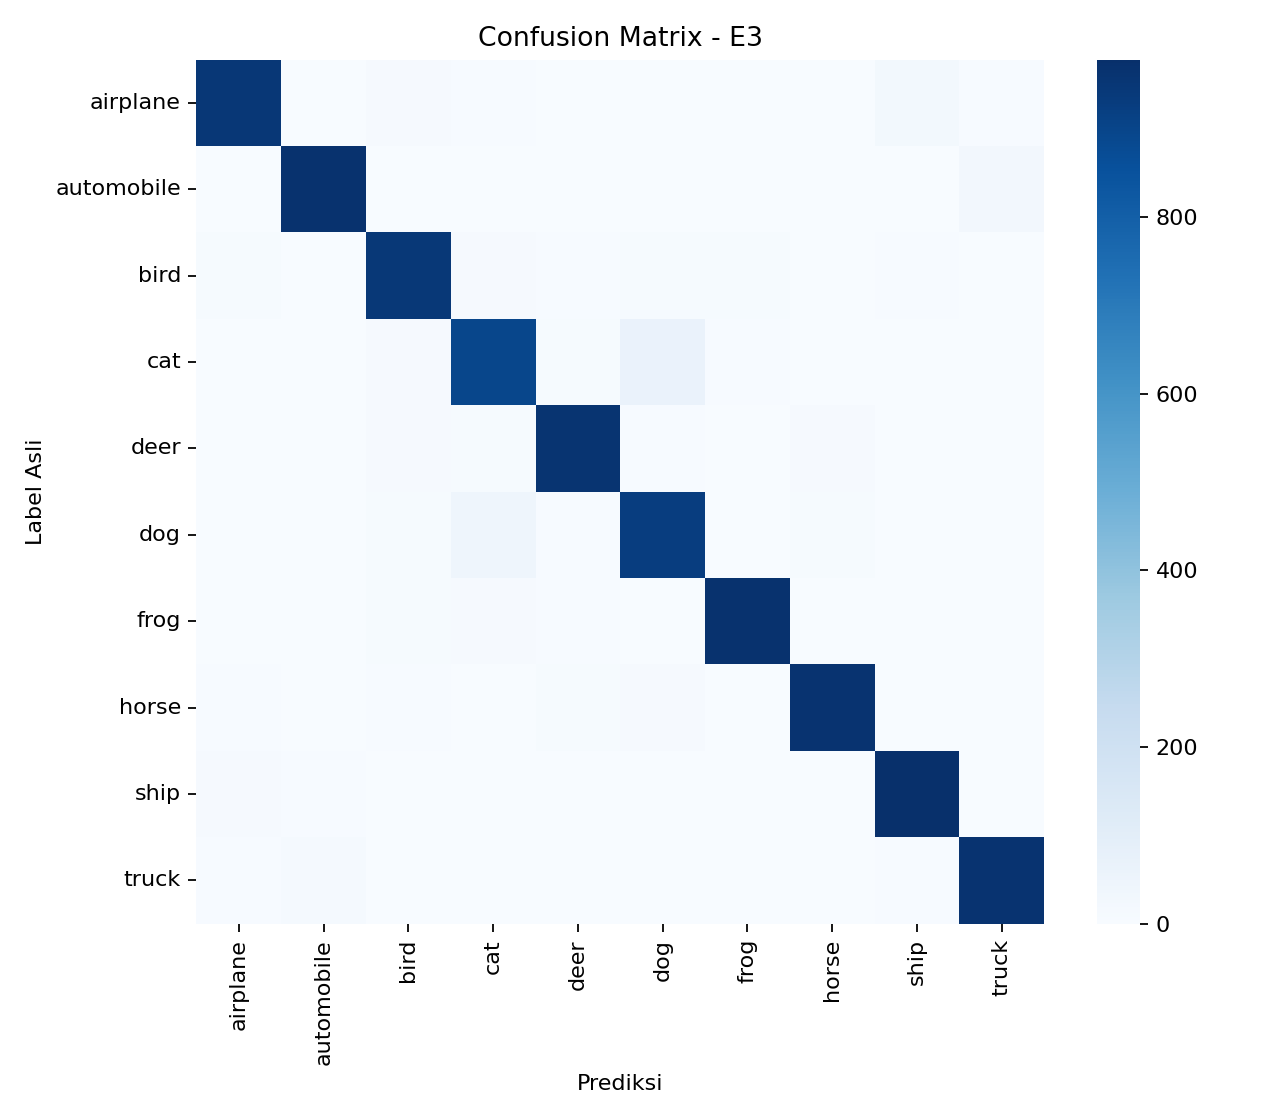
\includegraphics[width=0.92\columnwidth]{E3_confusion_matrix.png}
\caption{Confusion matrix E3 (ResNet-18 transfer learning). Diagonal yang dominan menunjukkan kesalahan antarkelas yang relatif kecil.}
\label{fig:cm}
\end{figure}

Sebaliknya, confusion matrix E3 pada Gambar~\ref{fig:cm} hampir seluruhnya terkonsentrasi pada diagonal utama. Residual error yang masih terlihat terutama berasal dari kelas hewan yang secara visual berdekatan, seperti cat dan dog. Dengan demikian, transfer learning meningkatkan accuracy sekaligus mengurangi penyebaran kesalahan antarkelas.

\subsection{Discussion}
Perbedaan E1 dan E2 mengindikasikan bahwa perubahan regularisasi tidak otomatis mengatasi keterbatasan feature extraction pada CNN sederhana. Dropout dirancang untuk mengurangi co-adaptation [1], tetapi pada eksperimen ini model tanpa dropout tetap menghasilkan accuracy dan F1 yang sedikit lebih tinggi. Sebaliknya, E3 memperoleh keuntungan besar dari representasi pretrained dan residual learning [2], [3].

Dari sisi generalisasi, E1 dan E2 menunjukkan train-validation curves yang relatif berdekatan, sedangkan E3 memiliki gap yang lebih besar setelah performa validation mencapai puncak. Ini menunjukkan trade-off yang penting: model dengan kapasitas representasi lebih besar mampu mencapai performa test jauh lebih tinggi, tetapi juga lebih cepat memasuki kondisi overfitting ringan. Penggunaan early stopping menjadi komponen penting dalam menjaga generalisasi E3.

\section{Conclusion}
Penelitian ini membandingkan CNN baseline, CNN dengan dropout 0,5, dan ResNet-18 pretrained untuk klasifikasi CIFAR-10 melalui tiga skenario eksperimen. Hasil test menunjukkan E3 sebagai konfigurasi terbaik dengan accuracy dan F1 sebesar 95,22\%, dibandingkan E1 sebesar 68,92\% dan E2 sebesar 67,39\%.

Analisis training menunjukkan E1 dan E2 belajar relatif stabil tanpa overfitting berat, tetapi kapasitas representasinya terbatas. E2 tidak memberikan peningkatan terhadap baseline pada konfigurasi yang diuji. E3 menghasilkan performa jauh lebih baik melalui transfer learning, namun menunjukkan gejala overfitting ringan setelah sekitar epoch ke-7 dan kemudian dihentikan lebih awal berdasarkan validation loss.

Keterbatasan penelitian adalah penggunaan satu dataset dan tiga konfigurasi model. Penelitian berikutnya dapat menguji variasi learning rate, batch size, strategi freezing versus full fine-tuning, augmentation, serta backbone pretrained lain untuk menilai trade-off accuracy dan biaya komputasi.

\begin{thebibliography}{5}\footnotesize
\bibitem{srivastava2014} N. Srivastava, G. Hinton, A. Krizhevsky, I. Sutskever, and R. Salakhutdinov, ``Dropout: A simple way to prevent neural networks from overfitting,'' \emph{J. Mach. Learn. Res.}, vol. 15, no. 56, pp. 1929--1958, 2014.
\bibitem{pan2010} S. J. Pan and Q. Yang, ``A survey on transfer learning,'' \emph{IEEE Trans. Knowl. Data Eng.}, vol. 22, no. 10, pp. 1345--1359, Oct. 2010, doi: 10.1109/TKDE.2009.191.
\bibitem{he2016} K. He, X. Zhang, S. Ren, and J. Sun, ``Deep residual learning for image recognition,'' in \emph{Proc. IEEE Conf. Comput. Vis. Pattern Recognit. (CVPR)}, 2016, pp. 770--778, doi: 10.1109/CVPR.2016.90.
\bibitem{krizhevsky2009} A. Krizhevsky, ``Learning multiple layers of features from tiny images,'' Tech. Rep., Univ. Toronto, 2009.
\bibitem{kingma2015} D. P. Kingma and J. Ba, ``Adam: A method for stochastic optimization,'' in \emph{Proc. Int. Conf. Learn. Representations (ICLR)}, 2015.
\end{thebibliography}

\end{document}
